% !TEX program = xelatex
\documentclass[11pt,a4paper]{article}

\usepackage[french,provide=*]{babel}
\usepackage{fontspec}
\usepackage[a4paper,margin=2.4cm]{geometry}
\usepackage{amsmath,amssymb,mathtools,amsthm}
\usepackage{booktabs,tabularx,longtable,array}
\usepackage{enumitem}
\usepackage[dvipsnames]{xcolor}
\usepackage{listings}
\usepackage[most]{tcolorbox}
\usepackage{pgfplots}
\pgfplotsset{compat=1.18}
\usepackage{microtype}
\usepackage[colorlinks=true,linkcolor=MidnightBlue,urlcolor=MidnightBlue,citecolor=MidnightBlue]{hyperref}

\setlength{\parindent}{0pt}
\setlength{\emergencystretch}{3em}
\setlength{\parskip}{0.55em}
\renewcommand{\arraystretch}{1.25}
\setlist{itemsep=0.25em,topsep=0.3em}

% ---------- Notations ----------
\newcommand{\E}{\mathbb{E}}
\newcommand{\Var}{\operatorname{Var}}
\newcommand{\Cov}{\operatorname{Cov}}
\newcommand{\KPSS}{\mathrm{KPSS}}
\newcommand{\dto}{\xrightarrow{\;d\;}}
\newcommand{\lhat}{\hat\lambda^2}
\newcommand{\code}[1]{\texttt{#1}}

% ---------- Boites ----------
\newtcolorbox{retenir}{colback=MidnightBlue!5,colframe=MidnightBlue!70,
  title=À retenir,fonttitle=\bfseries,boxrule=0.6pt,arc=2pt}
\newtcolorbox{piege}{colback=BrickRed!5,colframe=BrickRed!70,
  title=Piège d'entretien,fonttitle=\bfseries,boxrule=0.6pt,arc=2pt,before upper=\raggedright}
\newtcolorbox{projet}{colback=ForestGreen!5,colframe=ForestGreen!70,
  title=Dans le projet,fonttitle=\bfseries,boxrule=0.6pt,arc=2pt}

\theoremstyle{definition}
\newtheorem{hyp}{Hypothèse}
\renewcommand{\thehyp}{A\arabic{hyp}}
\newtheorem{defi}{Définition}
\newtheorem{theo}{Théorème}

\lstset{basicstyle=\ttfamily\small,columns=fullflexible,keepspaces=true,
  backgroundcolor=\color{gray!8},frame=single,rulecolor=\color{gray!40},
  breaklines=true,language=Python,commentstyle=\color{gray},
  keywordstyle=\color{MidnightBlue},showstringspaces=false}

\title{\textbf{Le test KPSS appliqué au pairs trading}\\[0.3em]
\large Cours de préparation à l'entretien --- projet de statistical arbitrage}
\date{28 octobre 2026}
\author{}

\begin{document}
\maketitle

\begin{abstract}
Le KPSS teste l'hypothèse nulle « la série est stationnaire ». Dans le projet, c'est lui, bien plus que l'ADF, qui décide quelles paires survivent : sur les 148 spreads candidats, il en rejette 133, dont 29 que l'ADF jugeait stationnaires. Ce cours reprend la théorie complète en isolant chaque hypothèse, définit les concepts extérieurs (variance de long terme, théorème de Donsker, pont brownien, estimateur de Newey-West), puis applique le test aux données et au code du projet.
\end{abstract}

\tableofcontents

\section*{Notations}
\addcontentsline{toc}{section}{Notations}

\begin{center}
\begin{tabularx}{\textwidth}{@{}lX@{}}
\toprule
Symbole & Signification \\
\midrule
$n$ & taille de l'échantillon (nombre de jours) \\
$y_t$ & série testée (dans le projet : le spread $z_t = p^{(1)}_t - \beta\,p^{(2)}_t$) \\
$\bar y$ & moyenne empirique de $y_t$ \\
$e_t$ & résidu : $e_t = y_t - \bar y$ (version niveau) ou résidu de la droite des MCO (version tendance) \\
$S_t$ & somme partielle des résidus : $S_t = \sum_{i=1}^{t} e_i$ \\
$\eta$ & numérateur de la statistique : $\eta = n^{-2}\sum_{t=1}^{n} S_t^2$ \\
$\gamma_k$, $\hat\gamma_k$ & autocovariance d'ordre $k$ et son estimateur $\hat\gamma_k = n^{-1}\sum_{t=k+1}^{n} e_t e_{t-k}$ \\
$\lambda^2$, $\hat\lambda^2(\ell)$ & variance de long terme et son estimateur de Newey-West à $\ell$ retards \\
$\ell$ & bandwidth (nombre de retards de l'estimateur de Newey-West) \\
$r_t$, $u_t$, $\sigma_u^2$ & marche aléatoire, ses chocs, et leur variance \\
$\varepsilon_t$, $\sigma_\varepsilon^2$ & composante stationnaire et sa variance \\
$\rho$, $\nu_t$, $\sigma_\nu^2$ & coefficient AR(1), innovation de l'AR(1) et sa variance \\
$\theta$, $\sigma$ & paramètres de l'Ornstein-Uhlenbeck : $dX_t = \theta(\mu - X_t)\,dt + \sigma\,dW_t$ \\
$W(r)$, $V(r)$ & mouvement brownien standard et pont brownien sur $[0,1]$ \\
\bottomrule
\end{tabularx}
\end{center}

Attention : $\eta$ (numérateur du KPSS) et $\nu_t$ (innovation de l'AR(1)) sont deux objets différents.

% =====================================================================
\section{Pourquoi un test de stationnarité}

Un test statistique ne prouve que ce qu'il rejette. Le KPSS existe pour pouvoir \textbf{rejeter la stationnarité}, ce que l'ADF ne sait pas faire.

Un test contrôle l'erreur de première espèce $\alpha = \mathbb{P}(\text{rejeter } H_0 \mid H_0 \text{ vraie})$. Un rejet est donc une conclusion forte : on se trompe au plus dans $\alpha = 5\,\%$ des cas. Un non-rejet est une conclusion faible : il peut simplement venir d'un manque de puissance.

\begin{center}
\begin{tabularx}{\textwidth}{@{}lXX@{}}
\toprule
 & ADF / Phillips-Perron & KPSS \\
\midrule
$H_0$ & racine unitaire, $I(1)$ & stationnaire, $I(0)$ \\
$H_1$ & stationnaire & racine unitaire \\
Rejet = preuve forte de & stationnarité & non-stationnarité \\
Non-rejet = & pas assez de preuves de stationnarité & pas assez de preuves contre la stationnarité \\
Zone de rejet & queue gauche (statistique très négative) & queue droite (statistique grande) \\
\bottomrule
\end{tabularx}
\end{center}

\paragraph{Pourquoi c'est utile en pairs trading.} L'ADF a peu de puissance près de $\rho = 1$ (fiche de révision, \S5 : 13\,\% de rejet pour $\rho = 0{,}98$ et $T = 250$). Inversement, un spread qui « passe » l'ADF peut contenir une petite composante de marche aléatoire. Le KPSS attaque la question par l'autre bout : il cherche activement une dérive persistante.

\paragraph{Lecture conjointe} (tableau du \S4.4.6 des docs).

\begin{center}
\begin{tabularx}{\textwidth}{@{}llXX@{}}
\toprule
ADF & KPSS & Lecture & Dans \code{spread\_stationnarity()} \\
\midrule
rejette & ne rejette pas & stationnarité confirmée & paire conservée \\
ne rejette pas & rejette & racine unitaire confirmée & \code{CointError} (ADF) \\
rejette & rejette & conflit : forte persistance, rupture, tendance, bandwidth mal choisi & \code{CointError} (KPSS) \\
ne rejette pas & ne rejette pas & manque de puissance des deux côtés & \code{CointError} (ADF) \\
\bottomrule
\end{tabularx}
\end{center}

\begin{piege}
Ne pas dire « le KPSS ne rejette pas, donc le spread \emph{est} stationnaire ». Le KPSS ne prouve pas la stationnarité : il dit seulement que les données ne la contredisent pas au niveau choisi.
\end{piege}

\paragraph{Niveau du filtre combiné.} Exiger « ADF rejette \emph{et} KPSS ne rejette pas » ne donne pas un test de niveau $5\,\%$. Les deux statistiques sont calculées sur la même série et sont fortement dépendantes ; le niveau et la puissance du couple doivent être étudiés par simulation (\S\ref{sec:simu}).

% =====================================================================
\section{Le modèle KPSS et ses hypothèses}

Kwiatkowski, Phillips, Schmidt et Shin (1992) écrivent la série observée comme la somme d'une tendance déterministe, d'une marche aléatoire et d'une composante stationnaire :
\begin{equation}\label{eq:modele}
y_t = \xi\, t + r_t + \varepsilon_t, \qquad r_t = r_{t-1} + u_t, \qquad u_t \sim \text{iid}(0,\sigma_u^2).
\end{equation}
La valeur initiale $r_0$ est fixe : elle joue le rôle de la constante. Tout le test porte sur un seul paramètre, la variance $\sigma_u^2$ des chocs de la marche aléatoire :
\[
H_0 : \sigma_u^2 = 0 \quad \bigl(r_t \equiv r_0,\ y_t \text{ stationnaire autour de } r_0 + \xi t\bigr)
\qquad\text{contre}\qquad
H_1 : \sigma_u^2 > 0 .
\]
Sous $H_0$, la marche aléatoire est « éteinte ». Sous $H_1$, elle s'ajoute à $\varepsilon_t$ et rend la série $I(1)$. La version \emph{niveau} (\code{regression='c'}, celle du projet) impose $\xi = 0$ ; la version \emph{tendance} (\code{regression='ct'}) laisse $\xi$ libre.

\paragraph{D'où vient la statistique ?} Supposons $\varepsilon_t$ et $u_t$ gaussiens iid et notons $q^2 = \sigma_u^2/\sigma_\varepsilon^2$ le rapport signal/bruit. La matrice de covariance du vecteur $y$ vaut alors $\sigma_\varepsilon^2\,(I + q^2 V)$ avec $V_{ij} = \min(i,j)$. Le test du multiplicateur de Lagrange (test du score) de $q^2 = 0$ conduit à
\[
\frac{e^\top V e}{\hat\sigma_\varepsilon^2} = \frac{\sum_{t=1}^{n} S_t^2}{\hat\sigma_\varepsilon^2},
\]
car, pour des résidus centrés ($S_n = 0$), $e^\top V e = \sum_{t}\bigl(\sum_{s \ge t} e_s\bigr)^2 = \sum_t S_{t-1}^2$. Nyblom et Mäkeläinen (1983) ont montré que ce test est localement le plus puissant parmi les tests invariants. KPSS reprennent cette statistique et remplacent $\hat\sigma_\varepsilon^2$ par la variance de long terme $\lhat$ pour l'étendre aux erreurs autocorrélées.

\subsection{Les hypothèses, une par une}

\begin{hyp}[Forme additive]
$y_t$ = composante déterministe + marche aléatoire + composante $I(0)$, comme dans \eqref{eq:modele}.

\emph{Si elle est fausse :} le test reste interprétable comme « $I(0)$ contre $I(1)$ », mais sa puissance n'est plus optimale.
\end{hyp}

\begin{hyp}[Composante déterministe bien spécifiée]
Constante seule pour \code{'c'} ; constante et tendance linéaire pour \code{'ct'}.

\emph{Si elle est fausse :} une tendance oubliée ou une rupture de niveau gonflent les sommes partielles $S_t$ et entraînent un rejet à tort (Lee, Huang et Shin, 1997).
\end{hyp}

\begin{hyp}[Dépendance faible de $\varepsilon_t$]
$\E[\varepsilon_t] = 0$, moments d'ordre strictement supérieur à $2$ bornés, mélange fort (\emph{strong mixing}) avec coefficients sommables, comme chez Phillips et Perron (1988). L'hétéroscédasticité est tolérée ; l'hypothèse iid n'est \emph{pas} requise.

\emph{Si elle est fausse :} avec de la mémoire longue, la série n'est pas $I(1)$, mais le KPSS rejette quand même (il sert d'ailleurs de test de mémoire longue, Lee et Schmidt, 1996).
\end{hyp}

\begin{hyp}[Variance de long terme finie et strictement positive]
$0 < \lambda^2 < \infty$ (voir \S\ref{sec:lrv}).

\emph{Si elle est fausse :} $\lambda^2 = \infty$ correspond à la mémoire longue (cf.~A3) ; $\lambda^2 = 0$ correspond à une série sur-différenciée (racine unitaire dans la partie MA), et la normalisation dégénère.
\end{hyp}

\begin{hyp}[Estimateur convergent de $\lambda^2$]
Le bandwidth vérifie $\ell \to \infty$ et $\ell/n \to 0$ (voir \S\ref{sec:nw}).

\emph{Si elle est fausse :} $\ell$ trop petit $\Rightarrow$ $\lambda^2$ sous-estimé et sur-rejet ; $\ell$ trop grand $\Rightarrow$ perte de puissance. C'est \textbf{le} point faible pratique du test.
\end{hyp}

\begin{hyp}[Série observée, non estimée]
Les valeurs critiques $0{,}347 / 0{,}463 / 0{,}739$ supposent que $y_t$ est une donnée brute.

\emph{Si elle est fausse :} pour un spread construit avec un $\hat\beta$ estimé sur les mêmes données, la loi change. Il faut les valeurs de Shin (1994), soit $0{,}314$ à $5\,\%$ pour un régresseur (\S\ref{sec:shin}).
\end{hyp}

\begin{hyp}[Stabilité sur l'échantillon]
Pas de rupture du processus générateur.

\emph{Si elle est fausse :} même effet qu'en A2 : une rupture ressemble à de la non-stationnarité.
\end{hyp}

\begin{hyp}[Validité asymptotique]
Les valeurs critiques sont des limites quand $n \to \infty$, sans correction de petit échantillon.

\emph{Si elle est fausse :} la vitesse de convergence dépend de la persistance de $\varepsilon_t$. Plus $\rho$ est proche de $1$, plus il faut de données (\S\ref{sec:simu}).
\end{hyp}

\begin{retenir}
A2, A5, A6 et A7 sont les hypothèses que le projet met réellement à l'épreuve. Elles reviennent au \S\ref{sec:limites}.
\end{retenir}

% =====================================================================
\section{Sommes partielles : l'intuition de la statistique}

Le KPSS mesure la taille des écarts cumulés à la moyenne : petits si la série revient vite à sa moyenne, énormes si elle dérive.

\paragraph{Étape 1 : les résidus.} En version niveau, $e_t = y_t - \bar y$. En version tendance, $e_t$ est le résidu de la régression MCO de $y_t$ sur $(1, t)$.

\paragraph{Étape 2 : les sommes partielles.}
\[
S_t = \sum_{i=1}^{t} e_i, \qquad t = 1,\dots,n, \qquad S_n = 0 \quad (\text{les résidus sont centrés}).
\]
$S_t$ est l'écart cumulé à la moyenne. Un spread qui revient vite à sa moyenne alterne des $e_t$ positifs et négatifs qui se compensent : $S_t$ oscille près de $0$. Un spread qui passe des mois au-dessus de sa moyenne puis des mois en dessous accumule des $e_t$ de même signe : $S_t$ fait de grandes bosses.

\paragraph{Étape 3 : les ordres de grandeur.} C'est ce qui justifie la normalisation par $n^2$.

\begin{center}
\begin{tabular}{@{}lll@{}}
\toprule
 & Sous $H_0$ (stationnaire) & Sous $H_1$ (marche aléatoire) \\
\midrule
taille de $e_t$ & $O_p(1)$ & $O_p(\sqrt n)$ \\
taille de $S_t$ & $O_p(\sqrt n)$, car $\Var(S_t) \approx t\,\lambda^2$ & $O_p(n^{3/2})$ \\
$\sum_t S_t^2$ & $O_p(n^2)$ & $O_p(n^4)$ \\
$\eta = n^{-2}\sum_t S_t^2$ & $O_p(1)$, loi limite non dégénérée & $O_p(n^2)$ \\
$\eta / \hat\lambda^2(\ell)$ & $O_p(1)$, loi pivotale & $O_p(n/\ell)$, diverge si $\ell/n \to 0$ \\
\bottomrule
\end{tabular}
\end{center}

Sous $H_0$, la bonne échelle de $S_t$ n'est pas $\sigma_\varepsilon^2$ mais $\lambda^2$, la variance de long terme (\S\ref{sec:lrv}).

\begin{projet}
$S_t$ est exactement l'objet qu'utilise l'exposant de Hurst (\code{Hurst\_test()}, méthode R/S, docs \S4.9.2). Le R/S regarde l'\emph{étendue} $\max_t S_t - \min_t S_t$ ; le KPSS regarde la \emph{somme des carrés} $\sum_t S_t^2$. Les deux répondent à la même question : les écarts à la moyenne s'accumulent-ils ? La statistique R/S modifiée de Lo (1991) utilise d'ailleurs le même estimateur de Newey-West que le KPSS.
\end{projet}

% =====================================================================
\section{Concept extérieur : la variance de long terme}\label{sec:lrv}

La variance de long terme $\lambda^2$ est la variance d'une \emph{somme} de variables autocorrélées, ramenée à une observation. Pour le spread UNH-ELV, elle vaut environ $160$ fois la variance « ordinaire » $\gamma_0$.

\subsection{Définition}

Soit $(e_t)$ stationnaire, de moyenne nulle, d'autocovariances $\gamma_k = \Cov(e_t, e_{t-k})$. Développons la variance de la somme :
\[
\Var(S_n) = \sum_{i=1}^{n}\sum_{j=1}^{n}\gamma_{i-j} = n\,\gamma_0 + 2\sum_{k=1}^{n-1}(n-k)\,\gamma_k .
\]
En divisant par $n$ et en faisant tendre $n$ vers l'infini :

\begin{defi}[Variance de long terme]
\[
\lambda^2 = \lim_{n\to\infty}\frac{1}{n}\Var(S_n) = \sum_{k=-\infty}^{+\infty}\gamma_k = \gamma_0 + 2\sum_{k=1}^{\infty}\gamma_k .
\]
\end{defi}

Si les $e_t$ sont iid, $\gamma_k = 0$ pour $k \ge 1$ et $\lambda^2 = \gamma_0 = \sigma^2$ : on retrouve la variance usuelle. Avec de l'autocorrélation positive, les écarts de même signe s'additionnent et $\lambda^2 > \gamma_0$.

\subsection{Quatre lectures équivalentes}

\begin{enumerate}
\item \textbf{Variance par unité de temps de la somme} : $\Var(S_t) \approx t\,\lambda^2$ pour $t$ grand. C'est pourquoi $\lambda^2$, et non $\gamma_0$, est l'échelle des sommes partielles du KPSS.
\item \textbf{Précision de la moyenne} : $\Var(\bar e) \approx \lambda^2/n$. C'est le dénominateur d'un $t$-test sur une moyenne avec erreurs autocorrélées (écarts-types HAC).
\item \textbf{Fréquence zéro} : $\lambda^2 = 2\pi f(0)$, où $f$ est la densité spectrale de $e_t$. $\lambda^2$ mesure l'énergie des mouvements les plus lents, exactement ce qu'une marche aléatoire ferait exploser.
\item \textbf{Représentation MA($\infty$)} : si $e_t = \psi(L)\,\nu_t$ avec $\nu_t$ bruit blanc de variance $\sigma_\nu^2$, alors $\lambda^2 = \sigma_\nu^2\,\psi(1)^2$ : l'effet cumulé d'un choc, au carré.
\end{enumerate}

\subsection{Le cas AR(1), celui du spread}

Le modèle OU discrétisé du projet est un AR(1) : $e_t = \rho\,e_{t-1} + \nu_t$. Alors $\gamma_k = \rho^k\gamma_0$ et $\gamma_0 = \sigma_\nu^2/(1-\rho^2)$. En sommant la série géométrique :
\[
\lambda^2 = \gamma_0\Bigl(1 + 2\sum_{k\ge1}\rho^k\Bigr) = \gamma_0\,\frac{1+\rho}{1-\rho} = \frac{\sigma_\nu^2}{(1-\rho)^2}.
\]
En temps continu, pour un OU $dX_t = \theta(\mu - X_t)\,dt + \sigma\,dW_t$, on obtient de même $\lambda^2 = \sigma^2/\theta^2$.

\begin{projet}
\textbf{Chiffres UNH-ELV} (spread de Johansen, 2010--2023, $n = 3\,522$) :

\begin{tabular}{@{}ll@{}}
$\hat\rho$ (AR(1), spread centré) & $0{,}9875$ \\
demi-vie $-\ln 2/\ln\hat\rho$ & $55$ jours (\code{test\_pair.ipynb} : $55{,}1$ j) \\
$\hat\gamma_0$ & $282$ \$$^2$ \\
$\lambda^2$ via l'AR(1) : $\hat\sigma_\nu^2/(1-\hat\rho)^2$ & $\approx 46\,100$ \$$^2$ \\
$\lambda^2$ via l'OU : $\hat\sigma^2/\hat\theta^2$, $\hat\theta = 0{,}01258$, $\hat\sigma = 2{,}702$ & $\approx 46\,100$ \$$^2$ \\
rapport $\lambda^2/\gamma_0 = (1+\rho)/(1-\rho)$ & $\approx 160$ \\
\end{tabular}
\end{projet}

\paragraph{Taille d'échantillon effective.} Pour estimer la moyenne du spread, $n$ observations autocorrélées valent $n_{\text{eff}} = n\,\gamma_0/\lambda^2$ observations indépendantes. Pour UNH-ELV : $n_{\text{eff}} \approx 3\,522/160 \approx 22$. Quatorze ans de données quotidiennes ne contiennent qu'une vingtaine d'informations indépendantes sur le niveau moyen du spread. C'est la clé de toutes les difficultés des \S\ref{sec:nw} et \S\ref{sec:simu}.

% =====================================================================
\section{Concept extérieur : Donsker, brownien et pont brownien}\label{sec:donsker}

Sous $H_0$, la statistique KPSS converge vers l'intégrale du carré d'un pont brownien. Cette loi ne dépend d'aucun paramètre, d'où des valeurs critiques universelles : $0{,}347$ ($10\,\%$), $0{,}463$ ($5\,\%$), $0{,}739$ ($1\,\%$).

\subsection{Mouvement brownien et théorème de Donsker}

Un mouvement brownien standard $W(r)$, $r \in [0,1]$, est un processus continu, nul en $0$, à accroissements indépendants et gaussiens, avec $\Var W(r) = r$.

Le TCL usuel ne donne la loi limite que du point final $S_n/\sqrt n$. Le théorème de Donsker (TCL fonctionnel) donne celle de toute la trajectoire. Sous A3--A4, il reste vrai avec des erreurs dépendantes, à condition de normaliser par $\lambda$ et non par $\sigma_\varepsilon$ (Phillips, 1987) :

\begin{theo}[Donsker, erreurs faiblement dépendantes]
\[
\frac{1}{\lambda\sqrt n}\sum_{t=1}^{\lfloor rn\rfloor}\varepsilon_t \;\dto\; W(r), \qquad r \in [0,1].
\]
\end{theo}

C'est là que la variance de long terme entre en scène : elle est l'échelle naturelle des sommes partielles.

\subsection{Le centrage fabrique un pont brownien}

Le KPSS somme des résidus centrés $e_t = \varepsilon_t - \bar\varepsilon$, pas les $\varepsilon_t$ eux-mêmes. Donc
\[
S_{\lfloor rn\rfloor} = \sum_{t \le rn}\varepsilon_t - \frac{\lfloor rn\rfloor}{n}\sum_{t=1}^{n}\varepsilon_t
\quad\Longrightarrow\quad
\frac{S_{\lfloor rn\rfloor}}{\lambda\sqrt n} \;\dto\; W(r) - r\,W(1) \eqqcolon V(r).
\]
$V$ est un \textbf{pont brownien} : un brownien ramené à $0$ en $r = 1$, puisque $S_n = 0$. On a $\Var V(r) = r(1-r)$ et $\Cov\bigl(V(r),V(s)\bigr) = \min(r,s) - rs$.

\subsection{Loi limite de la statistique}

Le numérateur est une somme de Riemann. Par le théorème de l'application continue (si $f$ est continue et $X_n \dto X$, alors $f(X_n) \dto f(X)$) :
\[
\eta = \frac{1}{n^2}\sum_{t=1}^{n}S_t^2 = \frac{1}{n}\sum_{t=1}^{n}\Bigl(\frac{S_t}{\sqrt n}\Bigr)^2 \;\dto\; \lambda^2\int_0^1 V(r)^2\,dr,
\qquad\text{donc}\qquad
\KPSS = \frac{\eta}{\lhat} \;\dto\; \int_0^1 V(r)^2\,dr .
\]
Le $\lambda^2$ du numérateur et celui du dénominateur se simplifient, à condition que $\lhat$ soit convergent (A5). La loi limite est alors \textbf{pivotale} : elle ne dépend ni de $\sigma_\varepsilon$, ni de l'autocorrélation, ni des unités du spread.

\paragraph{Propriétés de la loi limite} (loi de Cramér--von Mises, la même que celle du test d'adéquation du même nom) :
\begin{itemize}
\item moyenne : $\E\int_0^1 V^2 = \int_0^1 r(1-r)\,dr = 1/6 \approx 0{,}167$ ;
\item décomposition de Karhunen--Loève : $\int_0^1 V(r)^2\,dr = \sum_{k\ge1} Z_k^2/(k^2\pi^2)$ avec $Z_k$ normales centrées réduites indépendantes. C'est une somme pondérée de $\chi^2(1)$, positive et asymétrique à droite, d'où un test unilatéral à droite ;
\item version tendance (\code{'ct'}) : le détendancement produit un pont brownien « de second niveau » $V_2$, de moyenne $1/15$. Le déterministe absorbe plus de variation lente, donc les valeurs critiques sont plus petites.
\end{itemize}

\begin{center}
\begin{tabular}{@{}lcccccc@{}}
\toprule
Version & Moyenne & $10\,\%$ & $5\,\%$ & $2{,}5\,\%$ & $1\,\%$ \\
\midrule
niveau \code{'c'} (projet) & $1/6$ & $0{,}347$ & $0{,}463$ & $0{,}574$ & $0{,}739$ \\
tendance \code{'ct'} & $1/15$ & $0{,}119$ & $0{,}146$ & $0{,}176$ & $0{,}216$ \\
\bottomrule
\end{tabular}
\end{center}

\paragraph{Vérification par simulation} ($20\,000$ bruits blancs, $n = 2\,000$, $\lambda$ connu) : moyenne $0{,}1666$ ; quantiles à $90/95/99\,\%$ : $0{,}347$, $0{,}458$, $0{,}754$. On retrouve les tables à l'erreur Monte-Carlo près.

\paragraph{Contraste avec l'ADF.} La loi de Dickey-Fuller est une fonctionnelle d'un brownien,
$\tfrac12\bigl[W(1)^2 - 1\bigr]\big/\bigl(\int_0^1 W^2\bigr)^{1/2}$, étudiée sous l'hypothèse de racine unitaire. Le KPSS utilise le pont brownien sous l'hypothèse de stationnarité. Les deux tests reposent sur Donsker, appliqué à des objets différents.

% =====================================================================
\section{Concept extérieur : estimer \texorpdfstring{$\lambda^2$}{lambda²} avec Newey-West}\label{sec:nw}

On estime $\lambda^2$ en sommant les premières autocovariances empiriques avec des poids décroissants (noyau de Bartlett). Tout se joue sur le bandwidth $\ell$ : pour les spreads du projet, statsmodels prend $\ell = 37$ alors qu'il en faudrait environ $300$.

\subsection{Pourquoi on ne peut pas « tout sommer »}

L'estimateur naïf remplace chaque $\gamma_k$ par $\hat\gamma_k = n^{-1}\sum_{t} e_t e_{t-k}$ et somme tous les retards. Or, pour des résidus centrés, cette somme est \textbf{identiquement nulle} :
\[
\sum_{k=-(n-1)}^{n-1}\hat\gamma_k = \frac{1}{n}\Bigl(\sum_{t=1}^{n}e_t\Bigr)^2 = 0 .
\]
De plus, les $\hat\gamma_k$ d'ordre élevé sont estimés sur peu de paires et sont très bruités. Il faut donc \textbf{tronquer} à $\ell$ retards, avec $\ell \to \infty$ et $\ell/n \to 0$ (A5). Mais la troncature brute $\hat\gamma_0 + 2\sum_{k\le\ell}\hat\gamma_k$ peut donner une variance négative.

\subsection{L'estimateur de Newey-West (1987)}

\[
\hat\lambda^2(\ell) = \hat\gamma_0 + 2\sum_{k=1}^{\ell}\Bigl(1 - \frac{k}{\ell+1}\Bigr)\hat\gamma_k .
\]
Les poids de Bartlett $w_k = 1 - k/(\ell+1)$ décroissent linéairement et garantissent $\hat\lambda^2(\ell) \ge 0$ : aux effets de bord près, $\hat\lambda^2(\ell)$ est la variance empirique des sommes de blocs de longueur $\ell+1$, divisée par $\ell+1$, et une variance ne peut pas être négative.

C'est mot pour mot la fonction \code{\_sigma\_est\_kpss} de statsmodels 0.14.6 (version de \code{model\_venv}) :
\begin{lstlisting}
s_hat = np.sum(resids ** 2)
for i in range(1, lags + 1):
    resids_prod = np.dot(resids[i:], resids[: nobs - i])
    s_hat += 2 * resids_prod * (1.0 - (i / (lags + 1.0)))
return s_hat / nobs
\end{lstlisting}

\subsection{L'arbitrage biais-variance}

\begin{itemize}
\item \textbf{Biais} : avec de l'autocorrélation positive, on oublie les $\gamma_k$ au-delà de $\ell$ et on sous-pondère les autres. $\hat\lambda^2(\ell)$ est \textbf{biaisé vers le bas}, d'autant plus que $\ell$ est petit devant la mémoire $1/(1-\rho)$.
\item \textbf{Variance} : chaque retard ajouté apporte du bruit ; la variance relative de $\hat\lambda^2(\ell)$ croît comme $\ell/n$.
\item \textbf{Optimum} (Andrews, 1991, noyau de Bartlett) : $\ell^* = 1{,}1447\,(\alpha\, n)^{1/3}$. Pour un AR(1), $\alpha = \dfrac{4\rho^2}{(1-\rho)^2(1+\rho)^2}$, qui explose quand $\rho \to 1$.
\end{itemize}

\subsection{Les règles de choix de \texorpdfstring{$\ell$}{l}, appliquées à \texorpdfstring{$n = 3\,522$}{n = 3522}}

\begin{center}
\begin{tabular}{@{}llc@{}}
\toprule
Règle & Formule & $\ell$ \\
\midrule
$\ell_4$ (KPSS 1992, docs \S4.4.5) & $\lfloor 4(n/100)^{1/4}\rfloor$ & $9$ \\
$\ell_{12}$, option \code{nlags='legacy'} & $\lceil 12(n/100)^{1/4}\rceil$ & $30$ \\
\code{nlags='auto'} (défaut, utilisé par le projet) & Hobijn, Franses et Ooms (1998) & $37$ \\
optimum d'Andrews, AR(1), $\hat\rho = 0{,}9875$ (UNH-ELV) & $1{,}1447\,(\alpha n)^{1/3}$ & $322$ \\
\bottomrule
\end{tabular}
\end{center}

\paragraph{La règle \code{auto} de statsmodels} (\code{\_kpss\_autolag}) est une version « plug-in » de Newey et West (1994) :
\begin{enumerate}
\item fenêtre pilote : $m = \lfloor n^{2/9}\rfloor$, soit $m = 6$ pour $n = 3\,522$ ;
\item $s_0 = \hat\gamma_0 + 2\sum_{k=1}^{m}\hat\gamma_k$ et $s_1 = 2\sum_{k=1}^{m}k\,\hat\gamma_k$ ;
\item $\ell = \bigl\lfloor 1{,}1447\,(s_1/s_0)^{2/3}\,n^{1/3}\bigr\rfloor$.
\end{enumerate}

\begin{piege}
\textbf{La règle \code{auto} sature.} Elle ne regarde que $m = 6$ autocorrélations. Quand $\rho \to 1$, $s_1/s_0 \to 42/13 \approx 3{,}23$, donc $\ell$ plafonne à environ $2{,}5\,n^{1/3}$, soit $38$ pour $n = 3\,522$. Elle ne distingue pas une demi-vie de $10$ jours d'une demi-vie de $100$ jours. C'est pourquoi presque toutes les paires du projet reçoivent $\ell = 37$ ($38$ pour les paires de change, $n = 3\,645$).
\end{piege}

\begin{center}
\begin{tabular}{@{}cccc@{}}
\toprule
$\rho$ & demi-vie & $\ell$ \code{auto} (statsmodels) & $\ell^*$ d'Andrews \\
\midrule
$0{,}90$ & $6{,}6$ j & $35$ & $78$ \\
$0{,}95$ & $13{,}5$ j & $36$ & $126$ \\
$0{,}973$ (SNPS-CDNS) & $25$ j & $37$ & $192$ \\
$0{,}987$ (UNH-ELV) & $53$ j & $37$ & $314$ \\
$0{,}99$ & $69$ j & $37$ & $374$ \\
\bottomrule
\end{tabular}
\end{center}

\paragraph{Conséquence chiffrée sur UNH-ELV.} Avec $\ell = 37$, $\hat\lambda^2(37) = 9\,349$, soit $33\,\hat\gamma_0$, alors que la vraie valeur est d'environ $160\,\gamma_0$. Newey-West ne capte qu'un cinquième de la variance de long terme, et la statistique KPSS est gonflée d'un facteur $5$ environ.

\paragraph{Et sous $H_1$ ?} Si la série est une marche aléatoire, $\hat\lambda^2(\ell)$ croît comme $\ell\,n$ et la statistique comme $n/\ell$. Un grand $\ell$ protège contre le sur-rejet sous $H_0$ mais tue la puissance sous $H_1$. Il n'existe pas de choix gratuit.

% =====================================================================
\section{La statistique complète et un calcul à la main}

\subsection{La formule}

\[
\boxed{\;\KPSS = \frac{\eta}{\hat\lambda^2(\ell)}, \qquad \eta = \frac{1}{n^2}\sum_{t=1}^{n}S_t^2, \qquad S_t = \sum_{i\le t}(y_i - \bar y)\;}
\]
Règle de décision : on rejette $H_0$ (stationnarité) si $\KPSS >$ valeur critique. Test unilatéral à droite.

\begin{piege}
Les docs du projet (\S4.4.3) notent $\hat\sigma_\varepsilon^2$ le dénominateur. Il s'agit bien de la \textbf{variance de long terme} estimée par Newey-West, $\hat\lambda^2(\ell)$, pas de la variance des résidus $\hat\gamma_0$. En entretien, dire « $\lambda^2$ » ou « variance de long terme » pour lever l'ambiguïté.
\end{piege}

\subsection{Ce que fait \texorpdfstring{\code{statsmodels.tsa.stattools.kpss}}{kpss}}

\begin{lstlisting}
resids = x - x.mean()                                  # regression='c'
nlags  = _kpss_autolag(resids, nobs)                   # nlags='auto' -> 37 ici
eta    = np.sum(resids.cumsum() ** 2) / (nobs ** 2)    # numerateur
s_hat  = _sigma_est_kpss(resids, nobs, nlags)          # lambda^2 de Newey-West
kpss_stat = eta / s_hat
p_value = np.interp(kpss_stat, crit, [0.10, 0.05, 0.025, 0.01])
return kpss_stat, p_value, nlags, crit_dict
\end{lstlisting}

\subsection{Calcul pas à pas sur le spread Johansen UNH-ELV (2010--2023)}

\begin{center}
\begin{tabular}{@{}ll@{}}
\toprule
Étape & Valeur \\
\midrule
$n$ & $3\,522$ jours \\
spread & $\text{UNH}_t - 1{,}100\times\text{ELV}_t$ (prix, vecteur de Johansen) \\
$\hat\gamma_0$ & $282{,}3$ \$$^2$ \\
$\eta = n^{-2}\sum_t S_t^2$ & $2\,510{,}2$ \$$^2$ \\
$\ell$ choisi par \code{auto} & $37$ \\
$\hat\lambda^2(37)$ & $9\,348{,}8$ \$$^2$ \\
$\KPSS = \eta/\hat\lambda^2(37)$ & $\mathbf{0{,}269}$ (sans unité : les \$$^2$ se simplifient) \\
valeurs critiques & $0{,}347$ ($10\,\%$) ; $0{,}463$ ($5\,\%$) ; $0{,}739$ ($1\,\%$) \\
décision à $5\,\%$ & on ne rejette pas $H_0$ \\
$p$-value renvoyée & $0{,}10$, avec un \code{InterpolationWarning} \\
\bottomrule
\end{tabular}
\end{center}

Si l'on divisait $\eta$ par $\hat\gamma_0$ au lieu de $\hat\lambda^2(37)$, on obtiendrait $2\,510/282 \approx 8{,}9$ : un rejet massif. Toute la différence vient de la correction d'autocorrélation.

\subsection{Lire la \texorpdfstring{$p$}{p}-value correctement}

La $p$-value de statsmodels est une \textbf{interpolation linéaire} dans une table à quatre points ; elle est donc bornée à $[0{,}01\,;\,0{,}10]$. Une $p$-value affichée à $0{,}10$ signifie « $\ge 0{,}10$ » ; à $0{,}01$, elle signifie « $\le 0{,}01$ ». C'est le sens exact du message \emph{« The actual p-value is greater than the p-value returned »} vu dans \code{validation\_stat.ipynb} et \code{validation\_stat2.ipynb}. Le projet filtre ce message dans \code{test\_pair.ipynb}, ce qui est sans danger : la décision repose sur la statistique comparée à la valeur critique, pas sur la $p$-value.

% =====================================================================
\section{Taille et puissance : ce que montrent les simulations}\label{sec:simu}

Sur un spread stationnaire de demi-vie $53$ jours ($\rho = 0{,}987$) observé sur $3\,522$ jours, le KPSS de statsmodels rejette à tort la stationnarité \textbf{$56\,\%$ du temps} au lieu de $5\,\%$. Toutes les simulations sont des AR(1) gaussiens ($300$ tirages par case ; erreur Monte-Carlo d'environ $\pm 3$ points).

\subsection{Taille réelle sous \texorpdfstring{$H_0$}{H0}, \texorpdfstring{$n = 3\,522$}{n = 3522}, niveau nominal \texorpdfstring{$5\,\%$}{5\%}}

\begin{center}
\begin{tabular}{@{}lccccc@{}}
\toprule
$\rho$ & demi-vie & $\ell$ \code{auto} & $\ell = 37$ & $\ell = 100$ & $\ell = 300$ \\
\midrule
$0$ (bruit blanc) & -- & $6\,\%$ & $3\,\%$ & $8\,\%$ & $2\,\%$ \\
$0{,}5$ & $1$ j & $6\,\%$ & $4\,\%$ & $6\,\%$ & $4\,\%$ \\
$0{,}9$ & $6{,}6$ j & $10\,\%$ & $12\,\%$ & $6\,\%$ & $3\,\%$ \\
$0{,}95$ & $13{,}5$ j & $16\,\%$ & $15\,\%$ & $9\,\%$ & $4\,\%$ \\
$0{,}973$ (SNPS-CDNS) & $25$ j & $33\,\%$ & $32\,\%$ & $16\,\%$ & $5\,\%$ \\
$0{,}987$ (UNH-ELV) & $53$ j & $\mathbf{56\,\%}$ & $57\,\%$ & $22\,\%$ & $9\,\%$ \\
$0{,}991$ (EMR-ROK, VRSK-MCO) & $77$ j & $\mathbf{71\,\%}$ & $74\,\%$ & $32\,\%$ & $15\,\%$ \\
\bottomrule
\end{tabular}
\end{center}

La distorsion vient d'un $\ell$ trop petit devant la mémoire $1/(1-\rho)$ du processus. Avec $\ell = 300$, proche de l'optimum d'Andrews, la taille revient près de $5\,\%$ jusqu'à $\rho = 0{,}973$.

\subsection{Le sur-rejet diminue avec \texorpdfstring{$n$}{n}, mais lentement}

Pour $\rho = 0{,}987$ et $\ell$ \code{auto} : $75\,\%$ de rejet pour $n = 250$ ($\ell = 10$), $72\,\%$ pour $n = 1\,000$ ($\ell = 19$), $52\,\%$ pour $n = 3\,522$ ($\ell = 37$), $40\,\%$ pour $n = 10\,000$ ($\ell = 58$). Le test est asymptotiquement correct, mais $\ell$ ne croît qu'en $n^{1/3}$.

\begin{piege}
La phrase des docs (\S4.4.7) « sur-rejet en grande taille d'échantillon » mélange deux phénomènes :
\begin{enumerate}
\item \textbf{Distorsion de taille due à la persistance} : c'est un défaut du test, et elle \emph{diminue} quand $n$ augmente.
\item \textbf{Consistance contre de petites déviations} : $H_0$ impose $\sigma_u^2 = 0$ \emph{exactement}. Si les données réelles contiennent une infime dérive, le KPSS finit par la détecter quand $n$ grandit. Ce n'est pas un défaut : le test fait son travail sur une hypothèse nulle très stricte.
\end{enumerate}
\end{piege}

\subsection{Puissance sous \texorpdfstring{$H_1$}{H1} (marche aléatoire pure)}

\begin{center}
\begin{tabular}{@{}lcccc@{}}
\toprule
$n$ & $\ell$ \code{auto} & $\ell = 5$ & $\ell = 37$ & $\ell = 100$ \\
\midrule
$250$ & $82\,\%$ ($\ell = 10$) & $95\,\%$ & $56\,\%$ & $0\,\%$ \\
$1\,000$ & $96\,\%$ ($\ell = 19$) & $100\,\%$ & $90\,\%$ & $67\,\%$ \\
$3\,522$ & $100\,\%$ ($\ell = 38$) & $100\,\%$ & $100\,\%$ & $92\,\%$ \\
\bottomrule
\end{tabular}
\end{center}

Pour $n = 3\,522$, la statistique médiane vaut $32{,}3$ ($\ell = 5$), $4{,}2$ ($\ell = 37$) et $1{,}8$ ($\ell = 100$) : elle décroît comme $n/\ell$.

\subsection{Puissance contre une petite composante de marche aléatoire}

Modèle $y_t = r_t + \varepsilon_t$ avec $\varepsilon_t$ bruit blanc et $q = \sigma_u/\sigma_\varepsilon$, $n = 1\,000$ :

\begin{center}
\begin{tabular}{@{}lcccc@{}}
\toprule
$q = \sigma_u/\sigma_\varepsilon$ & $0$ & $0{,}01$ & $0{,}03$ & $0{,}1$ \\
\midrule
rejet à $5\,\%$ & $7\,\%$ & $59\,\%$ & $92\,\%$ & $96\,\%$ \\
\bottomrule
\end{tabular}
\end{center}

Une dérive dont les chocs sont $100$ fois plus petits que le bruit est détectée plus d'une fois sur deux. C'est le régime d'alternatives locales étudié par KPSS ($\sigma_u^2/\sigma_\varepsilon^2$ de l'ordre de $1/n^2$). Pour un trader, c'est exactement le risque à surveiller : une relation de cointégration qui se détériore lentement.

\subsection{Le filtre combiné ADF + KPSS du projet}

AR(1) stationnaires, $n = 3\,522$, règles exactes de \code{spread\_stationnarity()} :

\begin{center}
\begin{tabular}{@{}cccc@{}}
\toprule
$\rho$ & $\mathbb{P}(\text{ADF rejette})$ & $\mathbb{P}(\text{KPSS ne rejette pas})$ & $\mathbb{P}(\text{passe les deux})$ \\
\midrule
$0{,}973$ & $100\,\%$ & $70\,\%$ & $70\,\%$ \\
$0{,}987$ & $100\,\%$ & $47\,\%$ & $47\,\%$ \\
$0{,}991$ & $99{,}7\,\%$ & $32\,\%$ & $32\,\%$ \\
\bottomrule
\end{tabular}
\end{center}

\begin{retenir}
Avec $14$ ans de données, l'ADF n'est plus le goulot : $n(1-\rho) \approx 46$ suffit à lui donner toute sa puissance. \textbf{C'est le KPSS qui décide}, et il élimine plus de la moitié des spreads réellement stationnaires de demi-vie $50$ à $80$ jours. Le filtre est très conservateur : peu de faux positifs, beaucoup de faux négatifs.
\end{retenir}

% =====================================================================
\section{Le KPSS dans le projet}\label{sec:projet}

Les chiffres ci-dessous sont recalculés avec la logique de \code{Coint\_verif}, sur \code{financial\_datas.csv} (2010--2023) et sur \code{backtest\_datas.csv} (2024--2026).

\subsection{Où il est utilisé}

\begin{center}
\begin{tabularx}{\textwidth}{@{}lX@{}}
\toprule
Fichier & Usage \\
\midrule
\code{docs/04\_Validation\_statistique.md} \S4.4, \S4.11, \S4.13 & théorie, protocole : « KPSS sur $z_t$ : ne doit PAS rejeter $H_0$ » \\
\code{test\_coint.py}, l.~3 et 84--87 & filtre de \code{spread\_stationnarity()} \\
\code{validation\_stat2.ipynb}, cellules 12--13 & KPSS sur $x_t$ et sur $\Delta x_t$ \\
\code{validation\_stat.ipynb}, cellule 32 & KPSS sur le spread de Johansen synthétique \\
\code{answer.md}, Q016 et Q056 & réponses préparées \\
\bottomrule
\end{tabularx}
\end{center}

\subsection{Ce que montrent les notebooks}

Données simulées : $x_t = w_t + \varepsilon_t$ avec $w_t$ marche aléatoire de chocs $\mathcal N(0,1)$ et $\varepsilon_t \sim \mathcal N(0, 0{,}5^2)$, $n = 200$. C'est \textbf{exactement le modèle KPSS sous $H_1$}, avec $q = \sigma_u/\sigma_\varepsilon = 2$.

\begin{center}
\begin{tabularx}{\textwidth}{@{}lccX@{}}
\toprule
Série & KPSS & ADF & Lecture \\
\midrule
$x_t$ (cellule 12) & $0{,}689$ & $-2{,}50$ ($p = 0{,}12$) & KPSS rejette à $10$, $5$ et $2{,}5\,\%$, pas à $1\,\%$ ($0{,}739$) ; l'ADF ne rejette pas : $I(1)$ \\
$\Delta x_t$ (cellule 13) & $0{,}181$ & $-5{,}12$ & stationnaire, donc $x_t$ est $I(1)$ \\
$x_t - 0{,}670\,y_t$ (Johansen) & $0{,}055$ & -- & très loin sous $0{,}347$ ; $p$-value affichée $0{,}10$ = « $\ge 0{,}10$ » \\
\bottomrule
\end{tabularx}
\end{center}

Le rejet de $x_t$ dépend du niveau choisi : avec \code{crit\_level='1\%'}, ce même $x_t$ aurait passé le KPSS. Le spread synthétique vaut $x_t - 0{,}670\,y_t \approx -0{,}005\,w_t + \text{bruit}$ : c'est presque un bruit blanc, d'où la statistique minuscule.

\subsection{Le code de production}

\begin{lstlisting}
# test_coint.py, Coint_verif.spread_stationnarity()
stat, pvalue, lags, crit = kpss(spread, regression='c')
if stat >= crit[crit_level]:
    raise CointError("... pas stationnaire ... pour le test KPSS !")
\end{lstlisting}

\begin{itemize}
\item \code{regression='c'} est le bon choix : le modèle OU suppose un spread qui oscille autour d'une constante $\mu$. Un \code{'ct'} accepterait des spreads qui dérivent linéairement, ce qu'on ne veut pas trader.
\item \code{nlags} n'est pas précisé : c'est \code{'auto'}, donc $\ell = 37$ pour presque toutes les paires.
\item \code{crit} a pour clés \code{'10\%'}, \code{'5\%'}, \code{'2.5\%'}, \code{'1\%'} : les trois valeurs de \code{crit\_level} prévues par la docstring fonctionnent.
\item la décision ne regarde que la statistique ; \code{pvalue} et \code{lags} ne sont pas utilisés (on pourrait journaliser \code{lags}).
\item le spread testé est le spread de Johansen \textbf{en prix}, avec un $\hat\beta$ estimé sur les mêmes données (\S\ref{sec:shin}).
\end{itemize}

\begin{piege}
Hors KPSS, mais dans le même pipeline : \code{test\_batterie()} appelle \code{self.spread\_n\_hedge\_ratio()} alors que c'est une \code{@property}. L'expression renvoie un tuple puis tente de l'appeler, d'où un \code{TypeError}, non intercepté par \code{except CointError} dans \code{test\_pair.ipynb}. Il faut écrire \code{s, beta = self.spread\_n\_hedge\_ratio}, sans parenthèses.
\end{piege}

\subsection{Résultats sur l'univers de paires}

Sur \code{pairs\_universe.csv}, $149$ paires sont testables et $148$ passent l'étape $I(1)$. Croisement des deux tests sur leur spread de Johansen ($5\,\%$) :

\begin{center}
\begin{tabular}{@{}lcc@{}}
\toprule
 & KPSS ne rejette pas & KPSS rejette \\
\midrule
\textbf{ADF rejette} & $10$ & $29$ \\
\textbf{ADF ne rejette pas} & $5$ & $104$ \\
\bottomrule
\end{tabular}
\end{center}

\begin{itemize}
\item Le KPSS rejette $133$ spreads sur $148$ ($90\,\%$).
\item $29$ paires que l'ADF jugeait stationnaires sont éliminées par le seul KPSS, dont KO-PEP ($0{,}510$), LMT-RTX ($0{,}468$), CME-ICE ($0{,}476$) et GS-MS ($0{,}722$).
\item Parmi les $10$ survivantes, Engle-Granger et Johansen retirent HYG-JNK et CCI-SBAC. Il reste les $8$ paires de \code{test\_pair.ipynb}.
\end{itemize}

\begin{center}
\begin{tabular}{@{}lccccl@{}}
\toprule
Paire & $\hat\rho$ & demi-vie & ADF & KPSS ($\ell = 37$) & marge sous $0{,}463$ \\
\midrule
SNPS-CDNS & $0{,}973$ & $25$ j & $-6{,}00$ & $0{,}110$ & large \\
VRSK-MCO & $0{,}991$ & $81$ j & $-3{,}84$ & $0{,}167$ & large \\
DE-AGCO & $0{,}986$ & $49$ j & $-3{,}82$ & $0{,}206$ & large \\
ADP-PAYX & $0{,}989$ & $64$ j & $-4{,}04$ & $0{,}233$ & confortable \\
UNH-ELV & $0{,}988$ & $55$ j & $-3{,}98$ & $0{,}269$ & confortable \\
TMO-DHR & $0{,}990$ & $69$ j & $-3{,}80$ & $0{,}398$ & faible \\
ALL-TRV & $0{,}991$ & $76$ j & $-4{,}01$ & $\mathbf{0{,}460}$ & $0{,}003$ \\
EMR-ROK & $0{,}991$ & $80$ j & $-3{,}90$ & $\mathbf{0{,}459}$ & $0{,}004$ \\
\bottomrule
\end{tabular}
\end{center}

ALL-TRV et EMR-ROK passent à $0{,}003$ près, alors que KO-PEP ou LMT-RTX, de profil très proche, sont écartées. La frontière est quasi aléatoire : c'est la conséquence directe des simulations (à $\rho \approx 0{,}99$, la probabilité de rejet à tort est de l'ordre de $70\,\%$).

\subsection{Le verdict dépend du bandwidth}

\begin{itemize}
\item à $\ell = 10$, une seule des $8$ paires passe (SNPS-CDNS) ;
\item à $\ell = 20$ ou $30$, $5$ sur $8$ passent (UNH-ELV, DE-AGCO, SNPS-CDNS, ADP-PAYX, VRSK-MCO) ;
\item à $\ell = 37$, les $8$ passent ;
\item à $\ell = 100$, les $8$ passent, plus KO-PEP, LMT-RTX et CME-ICE ;
\item à $\ell \approx \ell^*$ d'Andrews ($320$ à $415$ selon la paire), UNH-ELV tombe à $0{,}068$, TMO-DHR à $0{,}093$, ALL-TRV à $0{,}094$, EMR-ROK à $0{,}138$ et KO-PEP à $0{,}136$.
\end{itemize}

\begin{center}
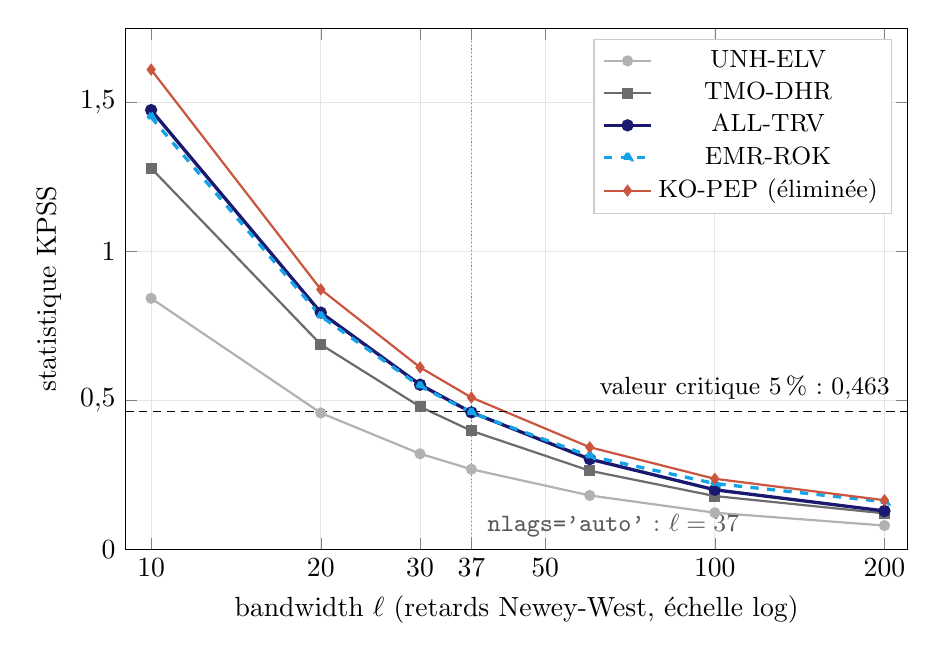
\begin{tikzpicture}
\begin{semilogxaxis}[
  width=0.95\textwidth, height=8.2cm,
  xlabel={bandwidth $\ell$ (retards Newey-West, échelle log)},
  ylabel={statistique KPSS},
  xmin=9, xmax=220, ymin=0, ymax=1.75,
  xtick={10,20,30,37,50,100,200},
  xticklabels={10,20,30,37,50,100,200},
  log ticks with fixed point,
  grid=major, grid style={gray!20},
  legend style={at={(0.98,0.98)},anchor=north east,font=\small,draw=gray!40},
  every axis plot/.append style={thick, mark size=1.6pt},
  /pgf/number format/use comma,
]
\addplot[gray!60, mark=*] coordinates {(10,0.843)(20,0.458)(30,0.321)(37,0.269)(60,0.181)(100,0.123)(200,0.080)};
\addlegendentry{UNH-ELV}
\addplot[gray!85!black, mark=square*] coordinates {(10,1.280)(20,0.688)(30,0.479)(37,0.398)(60,0.264)(100,0.179)(200,0.121)};
\addlegendentry{TMO-DHR}
\addplot[MidnightBlue, very thick, mark=*] coordinates {(10,1.475)(20,0.795)(30,0.553)(37,0.460)(60,0.303)(100,0.200)(200,0.129)};
\addlegendentry{ALL-TRV}
\addplot[Cerulean, very thick, dashed, mark=triangle*] coordinates {(10,1.451)(20,0.783)(30,0.548)(37,0.459)(60,0.313)(100,0.221)(200,0.160)};
\addlegendentry{EMR-ROK}
\addplot[BrickRed!70, mark=diamond*] coordinates {(10,1.611)(20,0.873)(30,0.611)(37,0.510)(60,0.343)(100,0.237)(200,0.165)};
\addlegendentry{KO-PEP (éliminée)}
\addplot[black, densely dashed, thin, forget plot] coordinates {(9,0.463)(220,0.463)};
\node[anchor=south west, font=\small] at (axis cs:60,0.47) {valeur critique $5\,\%$ : $0{,}463$};
\draw[gray, densely dotted] (axis cs:37,0) -- (axis cs:37,1.75);
\node[anchor=south west, font=\small, gray!70!black] at (axis cs:38,0.01) {\code{nlags='auto'} : $\ell = 37$};
\end{semilogxaxis}
\end{tikzpicture}

\small Calcul sur \code{financial\_datas.csv}, 2010--2023, spreads de Johansen, $n = 3\,522$.
\end{center}

Toutes les courbes décroissent à peu près comme $1/\ell$ : plus on prend de retards, plus $\hat\lambda^2(\ell)$ grossit et plus la statistique baisse. La liste finale de paires n'est donc pas une propriété des données seules : elle dépend d'un paramètre de lissage choisi par défaut par la librairie.

\subsection{Le spread est estimé : il faut les valeurs critiques de Shin}\label{sec:shin}

Le projet applique déjà ce raisonnement à l'ADF (docs \S4.6.1 et \S4.12.1) : un $\hat\beta$ estimé sur les mêmes données rend le résidu « trop stationnaire », d'où le recours à \code{coint()} et aux valeurs de MacKinnon. \textbf{Le même biais touche le KPSS, dans l'autre sens} : les sommes partielles $S_t$ sont artificiellement petites, et le test ne rejette pas assez. Shin (1994) a tabulé la loi correcte (test de l'hypothèse nulle de cointégration) :

\begin{center}
\begin{tabular}{@{}lccc@{}}
\toprule
Un régresseur + constante & $10\,\%$ & $5\,\%$ & $1\,\%$ \\
\midrule
Shin (1994) & $0{,}231$ & $0{,}314$ & $0{,}533$ \\
Simulation ($20\,000$ tirages, $n = 2\,000$) & $0{,}229$ & $0{,}314$ & $0{,}544$ \\
KPSS sur série brute (utilisé par le projet) & $0{,}347$ & $0{,}463$ & $0{,}739$ \\
\bottomrule
\end{tabular}
\end{center}

Avec $0{,}314$ à $5\,\%$, trois des $8$ paires tombent : TMO-DHR ($0{,}398$), ALL-TRV ($0{,}460$) et EMR-ROK ($0{,}459$).

\emph{Nuance :} Shin dérive sa loi pour un estimateur efficace de $\beta$ (moindres carrés dynamiques, avec avances et retards de $\Delta x_t$) qui neutralise l'endogénéité. Le $\hat\beta$ de Johansen est aussi efficace, mais ce n'est pas la procédure exacte de Shin : les seuils sont donc indicatifs.

\subsection{Stabilité dans le temps et hors échantillon}

\paragraph{Deux moitiés de l'échantillon} (2010--2016 / 2017--2023, $\hat\beta$ global) : UNH-ELV $0{,}777 / 0{,}749$ ; TMO-DHR $3{,}07 / 0{,}587$ ; ALL-TRV $4{,}04 / 0{,}926$ ; DE-AGCO $1{,}18 / 0{,}318$ ; ADP-PAYX $0{,}974 / 0{,}815$ ; EMR-ROK $1{,}33 / 0{,}547$ ; VRSK-MCO $0{,}743 / 0{,}361$. Seule SNPS-CDNS ($0{,}181 / 0{,}301$) passe sur les deux moitiés. Deux causes se cumulent : un $n$ plus petit aggrave la distorsion, et des changements de régime violent A7.

\paragraph{Hors échantillon} (janvier 2024 à juin 2026, $625$ jours, $\hat\beta$ estimé sur 2010--2023, $\ell$ \code{auto} $= 16$) :

\begin{center}
\begin{tabular}{@{}lccl@{}}
\toprule
Paire & KPSS & ADF & Lecture \\
\midrule
UNH-ELV & $0{,}426$ & $-2{,}01$ & ni KPSS ni ADF ne rejettent : non concluant \\
TMO-DHR & $1{,}612$ & $-1{,}92$ & non-stationnarité confirmée \\
DE-AGCO & $2{,}651$ & $-1{,}12$ & non-stationnarité confirmée \\
SNPS-CDNS & $2{,}896$ & $-0{,}78$ & non-stationnarité confirmée \\
\bottomrule
\end{tabular}
\end{center}

La relation s'est cassée pour trois des quatre paires backtestées. Et ce KPSS hors échantillon est indulgent : il recentre le spread sur sa moyenne 2024--2026, alors que la stratégie trade autour du $\hat\mu$ estimé sur 2010--2023. À mettre en regard des PnL de \code{image\_rapport/}.

\begin{retenir}
Un KPSS passé sur $14$ ans ne garantit rien sur les $2$ ans suivants. Il faut le refaire sur fenêtre glissante (docs \S8 : « Hebdo : tests ADF/KPSS »).
\end{retenir}

% =====================================================================
\section{Hypothèses violées dans le projet et améliorations}\label{sec:limites}

Quatre hypothèses du \S2 sont fragiles dans le projet : le bandwidth (A5), le $\hat\beta$ estimé (A6), la stabilité (A2/A7) et, plus marginalement, la variance non constante d'un spread en prix (A3).

\begin{center}
\small
\begin{tabularx}{\textwidth}{@{}>{\raggedright}p{2.1cm}>{\raggedright}X>{\raggedright}X>{\raggedright\arraybackslash}X@{}}
\toprule
Hypothèse & Situation dans le projet & Effet sur le test & Remède \\
\midrule
A5 & \code{auto} sature à $\ell = 37$ alors que $\ell^* \approx 300$ à $400$ & $\lambda^2$ sous-estimé d'un facteur $\approx 5$ ; rejet à tort de $50$ à $70\,\%$ des spreads de demi-vie $50$--$80$ j & $\ell$ d'Andrews, pré-blanchiment AR(1) (Andrews et Monahan, 1992), estimateur spectral autorégressif (Sul, Phillips et Choi, 2005), ou au minimum une analyse de sensibilité en $\ell$ \\
\addlinespace
A6 & spread construit avec un $\hat\beta$ de Johansen estimé sur les mêmes données & valeurs critiques trop indulgentes ($0{,}463$ au lieu de $0{,}314$) & valeurs de Shin (1994), ou bootstrap \\
\addlinespace
A2 / A7 & statistiques très différentes entre 2010--2016 et 2017--2023 ; rupture hors échantillon & une rupture de niveau ressemble à une racine unitaire & KPSS sur fenêtres glissantes, tests avec ruptures, réestimation périodique de $\beta$ et $\mu$ \\
\addlinespace
A3 & spread en \textbf{prix} (les docs parlent de log-prix) ; son échelle croît avec le niveau des actions & l'hétéroscédasticité est tolérée, mais une variance qui croît régulièrement pèse plus sur la fin de l'échantillon & log-prix ou spread normalisé \\
\addlinespace
Niveau du filtre & ADF et KPSS sur la même série ; $148$ paires testées & le couple n'a pas un niveau de $5\,\%$ ; tests multiples & assumer un filtre conservateur, contrôler le FDR (Benjamini-Hochberg), pré-filtre économique \\
\bottomrule
\end{tabularx}
\end{center}

\subsection{Corriger le bandwidth : le code et sa limite}

\begin{lstlisting}
e = spread - spread.mean()
rho = (e[1:] @ e[:-1]) / (e[:-1] @ e[:-1])
alpha = 4 * rho**2 / ((1 - rho)**2 * (1 + rho)**2)
l_opt = int(1.1447 * (alpha * len(e)) ** (1 / 3))   # 322 pour UNH-ELV
stat, p, lags, crit = kpss(spread, regression='c', nlags=l_opt)
\end{lstlisting}

\textbf{Limite à bien expliquer.} Sous $H_1$, $\hat\rho \to 1$, donc $\ell^*$ explose et la statistique s'effondre (simulation : $\ell = 100$ et $n = 250$ donnent $0\,\%$ de puissance). Même problème si l'on prend $\hat\lambda^2 = \hat\sigma^2/\hat\theta^2$ depuis le fit OU : sous $H_1$, $\hat\theta \to 0$ et la statistique tend vers $0$. Il faut donc \textbf{plafonner} $\ell$ (par exemple à $n/10$) ou plafonner $\hat\rho$, comme le proposent Sul, Phillips et Choi. Il n'existe pas de réglage gratuit : on arbitre entre faux rejets et puissance.

\subsection{Recommandations pour le projet}

\begin{enumerate}
\item \textbf{Utiliser les valeurs critiques de Shin} ($0{,}314$ à $5\,\%$) puisque le spread est estimé, par cohérence avec l'usage de \code{coint()} pour l'ADF.
\item \textbf{Rapporter la statistique pour plusieurs $\ell$} (\code{auto}, \code{legacy}, $\ell^*$ plafonné) et ne garder que les paires robustes à ce choix. ALL-TRV et EMR-ROK ne le sont pas.
\item \textbf{Tester la stabilité} : KPSS par sous-périodes ou sur fenêtre glissante d'un an, et hors échantillon avec le $\hat\mu$ d'estimation plutôt que la moyenne hors échantillon.
\item \textbf{Travailler en log-prix}, conformément aux docs (\S3), pour stabiliser la variance du spread.
\item \textbf{Garder l'esprit du filtre} : le KPSS est un détecteur de dérive lente, précisément le risque principal en pairs trading. Un rejet mérite une explication (persistance, rupture ou vraie racine unitaire) avant d'écarter la paire.
\end{enumerate}

% =====================================================================
\section{Questions d'entretien}

\begin{center}
\small
\begin{longtable}{@{}>{\raggedright}p{5.2cm}>{\raggedright\arraybackslash}p{10.3cm}@{}}
\toprule
Question & Réponse courte \\
\midrule
\endhead
Quelle est l'hypothèse nulle du KPSS ? & La stationnarité : $\sigma_u^2 = 0$, pas de composante marche aléatoire. C'est l'inverse de l'ADF. \\
\addlinespace
Pourquoi utiliser le KPSS en plus de l'ADF ? & Un test ne conclut fortement qu'en rejetant. L'ADF peut établir la stationnarité, le KPSS la non-stationnarité. Ensemble, ils distinguent « stationnaire » de « pas assez d'information ». \\
\addlinespace
Écrivez la statistique. & $\KPSS = \sum_t S_t^2 / \bigl(n^2\,\hat\lambda^2(\ell)\bigr)$, avec $S_t$ somme partielle des résidus centrés et $\hat\lambda^2(\ell)$ variance de long terme de Newey-West. \\
\addlinespace
Pourquoi $n^2$ ? & Sous $H_0$, $S_t = O_p(\sqrt n)$, donc $\sum_t S_t^2 = O_p(n^2)$. \\
\addlinespace
Pourquoi $\lambda^2$ et pas $\sigma_\varepsilon^2$ ? & Avec de l'autocorrélation, $\Var(S_t) \approx t\,\lambda^2$. Diviser par $\lambda^2$ rend la loi limite pivotale (Donsker avec erreurs dépendantes). \\
\addlinespace
Qu'est-ce que la variance de long terme ? & $\lambda^2 = \sum_k \gamma_k = \lim_n \Var(S_n)/n = 2\pi f(0)$. Pour un AR(1) : $\sigma_\nu^2/(1-\rho)^2$, soit $(1+\rho)/(1-\rho)$ fois $\gamma_0$ ; environ $160$ fois pour UNH-ELV. \\
\addlinespace
Quelle est la loi limite ? & $\int_0^1 V(r)^2\,dr$ avec $V(r) = W(r) - r\,W(1)$ pont brownien. Moyenne $1/6$. Seuil à $5\,\%$ : $0{,}463$ (niveau), $0{,}146$ (tendance). \\
\addlinespace
Pourquoi un pont brownien ? & Les résidus sont centrés, donc $S_n = 0$ : la trajectoire est ramenée à $0$ en $r = 1$. \\
\addlinespace
Pourquoi les poids de Bartlett ? & La troncature brute peut donner une variance négative. Les poids $1 - k/(\ell+1)$ garantissent $\hat\lambda^2(\ell) \ge 0$ : c'est une variance de sommes de blocs. \\
\addlinespace
Pourquoi ne pas sommer toutes les autocovariances ? & Pour des résidus centrés, $\sum_{|k|<n}\hat\gamma_k = 0$ exactement, et les $\hat\gamma_k$ lointains sont du pur bruit. \\
\addlinespace
Comment choisir $\ell$ ? & Arbitrage : $\ell$ petit $\Rightarrow$ sur-rejet sous $H_0$ ; $\ell$ grand $\Rightarrow$ perte de puissance (statistique en $n/\ell$ sous $H_1$). Règles $\ell_4$, $\ell_{12}$, Andrews (1991), Newey-West (1994). statsmodels : Hobijn et al.\ (1998), qui sature à $\approx 2{,}5\,n^{1/3}$. \\
\addlinespace
Quel $\ell$ dans le projet ? & $37$ pour presque toutes les paires (\code{nlags='auto'}, $n = 3\,522$), contre $\approx 320$ optimal pour UNH-ELV. \\
\addlinespace
Le KPSS est-il fiable pour un spread de demi-vie $55$ jours ? & Avec le réglage par défaut, non : $56\,\%$ de rejets à tort en simulation. ALL-TRV et EMR-ROK y passent à $0{,}003$ du seuil. \\
\addlinespace
Les valeurs critiques sont-elles les bonnes pour un spread estimé ? & Non. $\hat\beta$ rend le résidu trop stationnaire ; il faut Shin (1994) : $0{,}314$ à $5\,\%$ pour un régresseur. Trois des $8$ paires tomberaient. \\
\addlinespace
Que signifie une $p$-value de $0{,}10$ dans statsmodels ? & « $\ge 0{,}10$ » : la $p$-value est interpolée dans une table et bornée à $[0{,}01\,;\,0{,}10]$. \\
\addlinespace
ADF rejette et KPSS rejette : que conclure ? & Conflit : forte persistance (le cas typique ici), rupture, tendance non modélisée ou $\ell$ mal choisi. Le projet écarte la paire ; $29$ paires sont dans ce cas. \\
\addlinespace
« Le KPSS sur-rejette en grand échantillon » : vrai ? & À nuancer. La distorsion due à la persistance diminue avec $n$. Ce qui augmente, c'est la capacité à détecter de vraies petites dérives, car $H_0 : \sigma_u^2 = 0$ est très stricte. \\
\addlinespace
D'où vient la forme de la statistique ? & C'est le test du multiplicateur de Lagrange de $\sigma_u^2 = 0$ dans le modèle à composantes inobservées, localement le plus puissant (Nyblom et Mäkeläinen, 1983). \\
\addlinespace
Lien avec l'exposant de Hurst ? & Les deux reposent sur les sommes partielles centrées $S_t$ : R/S en regarde l'étendue, le KPSS la somme des carrés. \\
\addlinespace
Le KPSS validé en 2010--2023 tient-il en 2024--2026 ? & Pour $3$ paires backtestées sur $4$, non (statistiques de $1{,}6$ à $2{,}9$). Un test in-sample ne garantit pas la stabilité future. \\
\bottomrule
\end{longtable}
\end{center}

% =====================================================================
\section*{Sources}
\addcontentsline{toc}{section}{Sources}

\paragraph{Fichiers du projet relus.}
\begin{itemize}
\item \code{docs/04\_Validation\_statistique.md} ;
\item \code{docs/03\_Construction\_du\_spread.md} et \code{docs/08\_Roadmap\_implementation.md} ;
\item \code{test\_coint.py}, \code{Pair\_trading\_strat.py} ;
\item \code{validation\_stat.ipynb}, \code{validation\_stat2.ipynb}, \code{test\_pair.ipynb} ;
\item \code{answer.md} (Q014--Q016, Q056) et la fiche de révision sur les tests de racine unitaire ;
\item code source de \code{statsmodels.tsa.stattools.kpss} (0.14.6) et de \code{arch.unitroot.KPSS}.
\end{itemize}

\paragraph{Calculs.} Tous les chiffres sur données réelles sont recalculés à partir de \code{financial\_datas.csv}, \code{backtest\_datas.csv} et \code{pairs\_universe.csv} avec la logique de \code{Coint\_verif}. Les simulations utilisent des AR(1) gaussiens ($300$ tirages par configuration, $20\,000$ pour les lois limites).

\paragraph{Références} (citées de mémoire, non relues en ligne pour ce cours).
\begin{itemize}
\item Kwiatkowski, Phillips, Schmidt et Shin (1992), \emph{Testing the null hypothesis of stationarity against the alternative of a unit root}, Journal of Econometrics 54.
\item Nyblom et Mäkeläinen (1983), JASA : test LM de constance d'un niveau.
\item Phillips (1987), Econometrica : TCL fonctionnel avec erreurs dépendantes.
\item Newey et West (1987), Econometrica ; Newey et West (1994), Review of Economic Studies : estimateur HAC et choix automatique du bandwidth.
\item Andrews (1991), Econometrica ; Andrews et Monahan (1992) : bandwidth optimal, pré-blanchiment.
\item Hobijn, Franses et Ooms (1998 ; Statistica Neerlandica, 2004) : règle \code{auto} de statsmodels.
\item Shin (1994), Econometric Theory 10 : KPSS sur résidus de cointégration.
\item Lee, Huang et Shin (1997) : KPSS et ruptures structurelles. Lee et Schmidt (1996) : KPSS et mémoire longue.
\item Sul, Phillips et Choi (2005), Oxford Bulletin of Economics and Statistics : variance de long terme par pré-blanchiment borné.
\end{itemize}

\end{document}
